% !TEX spellcheck = en_US

%\documentclass[border=0.5]{standalone}
\documentclass[border=3mm]{standalone}

\usepackage{tikz}
%\usetikzlibrary{patterns,calc,angles,quotes,positioning,arrows}
\usetikzlibrary{math}
\usetikzlibrary{decorations.pathmorphing}
\usetikzlibrary{arrows.meta}

	% ======================================= V
	\newcommand{\stickman}[4]{% \stickman ==== V
		\draw[
			evaluate={
				\x = (#1); % center x
				\y = (#2); % center y
				\r = (#3); % radius
				\xl = \x-\r; % x left
				\xr = \x+\r; % x right
				\ya = \y-\r; % body upper
				\yb = \ya-\r; % arms
				\yc = \yb-\r; % legs
				\ybd = \yb-0.5*\r; % arms lower
				\ycd = \yc-0.5*\r; % legs lower
			},
			thick, orange
		]
		(\x, \y) circle (\r) % head
		(\x, \y) node {\textbf{#4}}
		(\x, \ya) -- (\x,\yc) % body
		(\xl, \ybd) -- (\x, \yb) -- (\xr, \ybd) %arms
		(\xl, \ycd) -- (\x, \yc) -- (\xr, \ycd) %arms
		; %
	} % \stickman ==== A
	% ======================================= A


% ======================================= A


\begin{document}


		% ======================================= V
		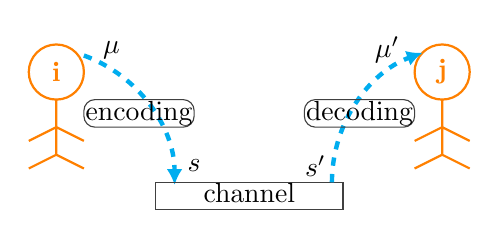
\begin{tikzpicture}[scale=0.7]
		%	% grid === V
		%	\draw[step=1.0,green,very thin] (0,0) grid (9,4);
		%	% ==== A
		
			\stickman{1}{3}{0.5}{i}
			\stickman{8}{3}{0.5}{j}

			
%			\uncover<2->{
				\node at (2, 3.4) {$\mu$};
%			}
				
%			\uncover<3->{
				% encoding
				\draw[-{Latex[length=2mm,width=2mm]},ultra thick,dashed, cyan]  
					(1.5,3.3) arc (70:0:2.5cm);
				\draw [rounded corners, darkgray] (1.5, 2) rectangle (3.5, 2.5);
				\node at (2.5, 2.25) {encoding};
				\node at (3.5, 1.3) {$s$};
%			}
			
%			\uncover<4->{
				% channel
				\draw [darkgray] (2.8, 1) rectangle (6.2,.5);
				\node at (4.5, 0.8) {channel};
				\node at (5.7, 1.3) {$s'$};
%			}
			
%			\uncover<5->{
				% decoding
				\draw[-{Latex[length=2mm,width=2mm]},ultra thick,dashed, cyan]  
					(6, 1) arc (180:110:2.5cm);
				\draw [rounded corners, darkgray] (5.5, 2) rectangle (7.5, 2.5);
				\node at (6.5, 2.25) {decoding};
				\node at (7, 3.4) {$\mu'$};
%			}
			
		\end{tikzpicture}
		% ======================================= A





%\newcommand{\stickman}[4]{% \stickman ==== V
%	\draw[
%		evaluate={
%			\x = (#1); % center x
%			\y = (#2); % center y
%			\r = (#3); % radius
%			\xl = \x-\r; % x left
%			\xr = \x+\r; % x right
%			\ya = \y-\r; % body upper
%			\yb = \ya-\r; % arms
%			\yc = \yb-\r; % legs
%			\ybd = \yb-0.5*\r; % arms lower
%			\ycd = \yc-0.5*\r; % legs lower
%		},
%		thick, orange
%	]
%	(\x, \y) circle (\r) % head
%	(\x, \y) node {\textbf{#4}}
%	(\x, \ya) -- (\x,\yc) % body
%	(\xl, \ybd) -- (\x, \yb) -- (\xr, \ybd) %arms
%	(\xl, \ycd) -- (\x, \yc) -- (\xr, \ycd) %arms
%	; %
%} % \stickman ==== A
%
%
%\begin{tikzpicture}
%%	% grid === V
%%	\draw[step=1.0,green,very thin] (0,0) grid (9,4);
%%	% ==== A
%
%	\stickman{1}{3}{0.5}{i}
%	\stickman{8}{3}{0.5}{j}
%	
%	% encoding
%	\draw [rounded corners, darkgray] (1.5, 2) rectangle (3.5, 2.5);
%	\node at (2.5, 2.25) {encoding};
%	\draw [<-,dashed, cyan] (3,1) arc (0:70:2.5cm);
%	\node at (2, 3.2) {$\mu$};
%	\node at (3.2, 1.2) {$s$};
%	
%	% channel
%	\draw [darkgray] (2.8, 1) rectangle (6.2,.6);
%	\node at (4.5, 0.8) {channel};
%
%	% decoding
%	\draw [rounded corners, darkgray] (5.5, 2) rectangle (7.5, 2.5);
%	\node at (6.5, 2.25) {decoding};
%	\draw [->,dashed, darkgray] (6, 1) arc (180:110:2.5cm);
%	\node at (7, 3.2) {$\mu'$};
%	\node at (5.8, 1.2) {$s'$};
%	
%\end{tikzpicture}

%\begin{frame}a few lines
%	\begin{center}
%	\begin{tikzpicture}
%		\draw [blue, ultra thick] (-1,2) -- (6,3);
%		\uncover<1>{\draw  [green,thick] (-4,3) -- (2,2.5);}
%		\uncover<2>{\draw  [red,thick] (0,0) -- (0,5);}
%	\end{tikzpicture}
%	\end{center}
%	and something under.
%\end{frame}

\end{document}